\documentclass[12pt]{article}

\setlength{\parindent}{0em}
\setlength{\parskip}{.5em}

\usepackage{framed}
\newcounter{problem}
\newcounter{problempart}[problem]
\newcounter{solutionpart}[problem]
\newenvironment{problem}{\stepcounter{problem}\noindent{\bf\arabic{problem}.}}{\setcounter{problempart}{0}\setcounter{solutionpart}{0}}
\newenvironment{solution}{\par\textcolor{blue}\bgroup}{\egroup\par}
\newcommand{\qpart}{\stepcounter{problempart}${}$\\\noindent{(\alph{problempart})} }
\newcommand{\spart}{\stepcounter{solutionpart}${}$\\\noindent{(\alph{solutionpart})} }
\newcommand{\TODO}{\textcolor{red}{$\blacksquare$}}
\newcommand{\SOL}[1]{\textcolor{blue}{#1}}
\usepackage{xspace}

\usepackage{hyperref}
\usepackage{fullpage}
\usepackage{amsmath,mathabx,MnSymbol}
\usepackage{color,tikz}
\usepackage{footnote,enumitem}
\usepackage{longtable}
\newcommand{\mx}[1]{\begin{pmatrix}#1\end{pmatrix}}
\definecolor{dkgreen}{rgb}{0,.5,0}
\usepackage{algorithm}
\usepackage[noend]{algpseudocode}

\newcommand{\uu}{\mathbf{u}}
\newcommand{\vv}{\mathbf{v}}
\newcommand{\cc}{\mathbf{c}}
\newcommand{\ww}{\mathbf{w}}
\newcommand{\xx}{\mathbf{x}}
\newcommand{\zz}{\mathbf{z}}
\newcommand{\MM}{\mathbf{M}}
\newcommand{\bb}{\mathbf{b}}
\newcommand{\ee}{\mathbf{e}}
\newcommand{\pp}{\mathbf{p}}
\newcommand{\qq}{\mathbf{q}}
\renewcommand{\AA}{\mathbf{A}}
\newcommand{\BB}{\mathbf{B}}
\newcommand{\CC}{\mathbf{C}}
\newcommand{\DD}{\mathbf{D}}
\newcommand{\nn}{\mathbf{n}}
\newcommand{\gp}[1]{\left(#1\right)}
\newcommand{\Bezier}{B\'ezier\xspace}
\newcommand{\dcj}{De Casteljau\xspace}

\newcommand{\TODOL}[1]{\textcolor{red}{\underline{\hspace{#1 cm}}}}

\usepackage{listings}

\lstset{
  language=C++,
  showstringspaces=false,
  identifierstyle=\color{magenta},
  basicstyle=\color{magenta},
  keywordstyle=\color{blue},
  identifierstyle=\color{black},
  commentstyle=\color{green},
  stringstyle=\color{red}
}

\begin{document}

\title{CS130 - Curves}
\date{}
\author{Name: \TODOL7\qquad\qquad SID: \TODOL4}
\maketitle
\begin{center}
\end{center}


\begin{center}
  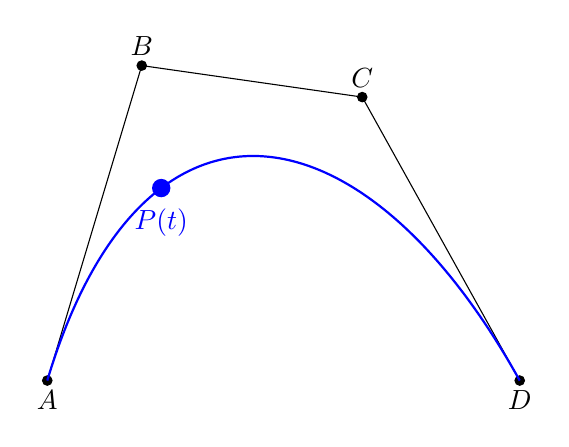
\begin{tikzpicture}[scale=2]
    \coordinate (A) at (0,0);
    \coordinate (B) at (.6,2);
    \coordinate (C) at (2,1.8);
    \coordinate (D) at (3,0);
    \draw[] (A) -- (B) -- (C) -- (D);
    \draw[fill=black] (A) node[below]{$A$} circle (.03);
    \draw[fill=black] (B) node[above]{$B$} circle (.03);
    \draw[fill=black] (C) node[above]{$C$} circle (.03);
    \draw[fill=black] (D) node[below]{$D$} circle (.03);
    \draw[thick,blue] (A) .. controls (B) and (C)  .. (D) node[pos=.3,circle,fill=blue,label=below:$P(t)$,inner xsep=0pt,outer xsep=0pt] {};
  \end{tikzpicture}
\end{center}

The following problems refer the figure above.  In these problems, we will be deriving the cubic  \Bezier from some of its properties.  This will help motivate the choices in the definition of the \Bezier curve.  Let $A$, $B$, $C$, and $D$ be the control points for the curve, and let $p_a(t)$, $p_b(t)$, $p_c(t)$, and $p_d(t)$ be the blending functions, so that $P(t) = p_a(t) A + p_b(t) B + p_c(t) C + p_d(t) D$.

The cubic \Bezier curve has the following properties:
\begin{enumerate}
\item Symmetry.  Reversing the order of $A,B,C,D$ results in the same curve, but with $t$ replaced with $1-t$. \label{prop:sym}
\item \Bezier curves end at two of the control points.  $P(0) = A$ and $P(1) = D$.\label{prop:ad}
\item The slope of the curve at the endpoints is given by the segment connecting the control points.  $P'(0) = k(B-A)$ and $P'(1) = k(C-D)$ for some $k$.\label{prop:slope}
\item Convex hull.  The \Bezier curve is inside the convex hull of the control points.\label{prop:hull}
\item The blending functions form a \textit{partition of unity}.  That is,
  $p_a(t)+p_b(t)+p_c(t)+p_d(t)=1$ for all $t$.  \label{prop:unity}
\end{enumerate}

\begin{problem}
  \Bezier curves are \textit{symmetrical}. Using property \ref{prop:sym}, express $p_a(t)$ and $p_b(t)$ as functions of $p_c(t)$ and $p_d(t)$.
\end{problem}

\begin{solution}
  \textbf{\textcolor{red}{\TODO}}
\end{solution}

\begin{problem}
  Since $p_c(t)$ and $p_d(t)$ are cubic polynomials, we can write them as
  \begin{align*}
    p_c(t) &= c_0 + c_1 t + c_2 t^2 + c_3 t^3 \\
    p_d(t) &= d_0 + d_1 t + d_2 t^2 + d_3 t^3
    \end{align*}
for some coefficients $c_0, \ldots, c_3$ and $d_0, \ldots, d_3$.
  Use property \ref{prop:ad} to solve for $c_0$, $d_0$, $c_3$, and $d_3$.  Use
  these to eliminate those variables from $p_c(t)$ and $p_d(t)$.
\end{problem}

\begin{solution}
  \textbf{\textcolor{red}{\TODO}}
\end{solution}

\begin{problem}
  Use property \ref{prop:slope} to solve for $c_1$, $d_1$, $c_2$, and $d_2$ as a
  function of $k$.  Eliminate those variables from $p_c(t)$ and $p_d(t)$.  These
  polynomials should now only depend on $t$ and $k$.
\end{problem}

\begin{solution}
  \textbf{\textcolor{red}{\TODO}}
\end{solution}

\begin{problem}
  Write out $p_a(t)$ and $p_b(t)$ as functions of $t$ and $k$.
\end{problem}

\begin{solution}
  \textbf{\textcolor{red}{\TODO}}
\end{solution}

\begin{problem}
  For \Bezier curves, $k=3$.  This choice is made because of property
  \ref{prop:hull}.  In particular, if $A=B$ (so that the convex hull is the
  triangle $BCD$), show that if $k>3$ then $P(t)$ is outside triangle $BCD$ for
  some $0 \le t \le 1$.  (Hint: the blending functions serve as barycentric
  weights.)
\end{problem}

\begin{solution}
  \textbf{\textcolor{red}{\TODO}}
\end{solution}

\begin{problem}
  For the case $k=3$, write out the blending functions.  Show that the \dcj
  algorithm produces the same point as $P(t)$.
\end{problem}

\begin{solution}
  \textbf{\textcolor{red}{\TODO}}
\end{solution}

\begin{problem}
  A set is called \textit{convex} if the segment connecting any two points in
  the set is itself entirely in the set.  Use the \dcj algorithm to show that
  the \Bezier curve is inside the convex hull of its control points.
\end{problem}

\begin{solution}
  \textbf{\textcolor{red}{\TODO}}
\end{solution}

\begin{problem}
  Let $\xx \to \MM \xx + \bb$ be an affine transformation, where $\MM$ is a
  matrix and $\bb$ is a vector.  Show that transforming the control points $A$,
  $B$, $C$, and $D$ is equivalent to transforming $P(t)$.  That is, we can
  transform a \Bezier curve by simply transforming its control points.
\end{problem}

\begin{solution}
  \textbf{\textcolor{red}{\TODO}}
\end{solution}

\begin{problem}
  The blending functions for the degree $n$ \Bezier curve are given by
  $$
p_k(t) = \mx{ n \\ k} t^k (1-t) ^{n-k}, \quad k = 0, \ldots, n
  $$
The binomial theorem states that
$$
(x + y)^n = \sum_{k=0}^n \mx{n \\ k} x^{n-k} y^k
$$
Letting $x = t$ and $y=1-t$ in the binomial theorem, show that the \Bezier blending functions satisfy property \ref{prop:unity}.
\end{problem}

\begin{solution}
  \textbf{\textcolor{red}{\TODO}}
\end{solution}

\pagebreak
\begin{problem}
\begin{center}
  \begin{tikzpicture}[scale=2]
n    \coordinate (a) at (-2,-2);
    \coordinate (b) at (2,-2);
    \coordinate (c) at (2,2);
    \coordinate (d) at (-2,2);
    \draw (a) node[label=below left:a] {};
    \draw (b) node[label=below right:b] {};
    \draw (c) node[label=above right:c] {};
    \draw (d) node[label=above left:d] {};
    \draw (a) -- (b) -- (c) -- (d) -- cycle;
    \coordinate (A) at (0,-2);
    \coordinate (D) at (-2,0);
    \draw (A) node[circle,fill=blue,label=below:A] {};
    \draw (D) node[circle,fill=blue,label=left:D] {};
  \end{tikzpicture}
\end{center}
Consider the figure above.  In this exercise, you will be drawing new control points and sketching the resulting \Bezier curves according to the instructions below.  We will refer to the edges of the square $abcd$ as e.g., edge $ab$, edge $bc$, etc.
\begin{enumerate}
\item Draw control points B and C so that the \Bezier curve $p_1(t)$, with control points ABCD, satisfies $p_1'(0)$ parallel to edge $ab$ and $p_1'(1)$ perpendicular to edge $ad$.
\item Sketch the \Bezier curve $p_1(t)$.
\item Place a new control points E and F so that the \Bezier curve $p_2(t)$, with control points DCEF, ends tangent to the edge $cd$.
\item Sketch the \Bezier curve $p_2(t)$.
\item Add two control points G and H so that the \Bezier curve $p_3(t)$, with control points by FGHA, is $C^1$ continuous with the \Bezier curves $p_1(t)$ and $p_2(t)$.
\item Sketch the \Bezier curve $p_3(t)$.
\end{enumerate}
\end{problem}

\begin{solution}
  \textbf{\textcolor{red}{\TODO}}
\end{solution}

\end{document}
